\begin{figure}[htbp]
  \centering
  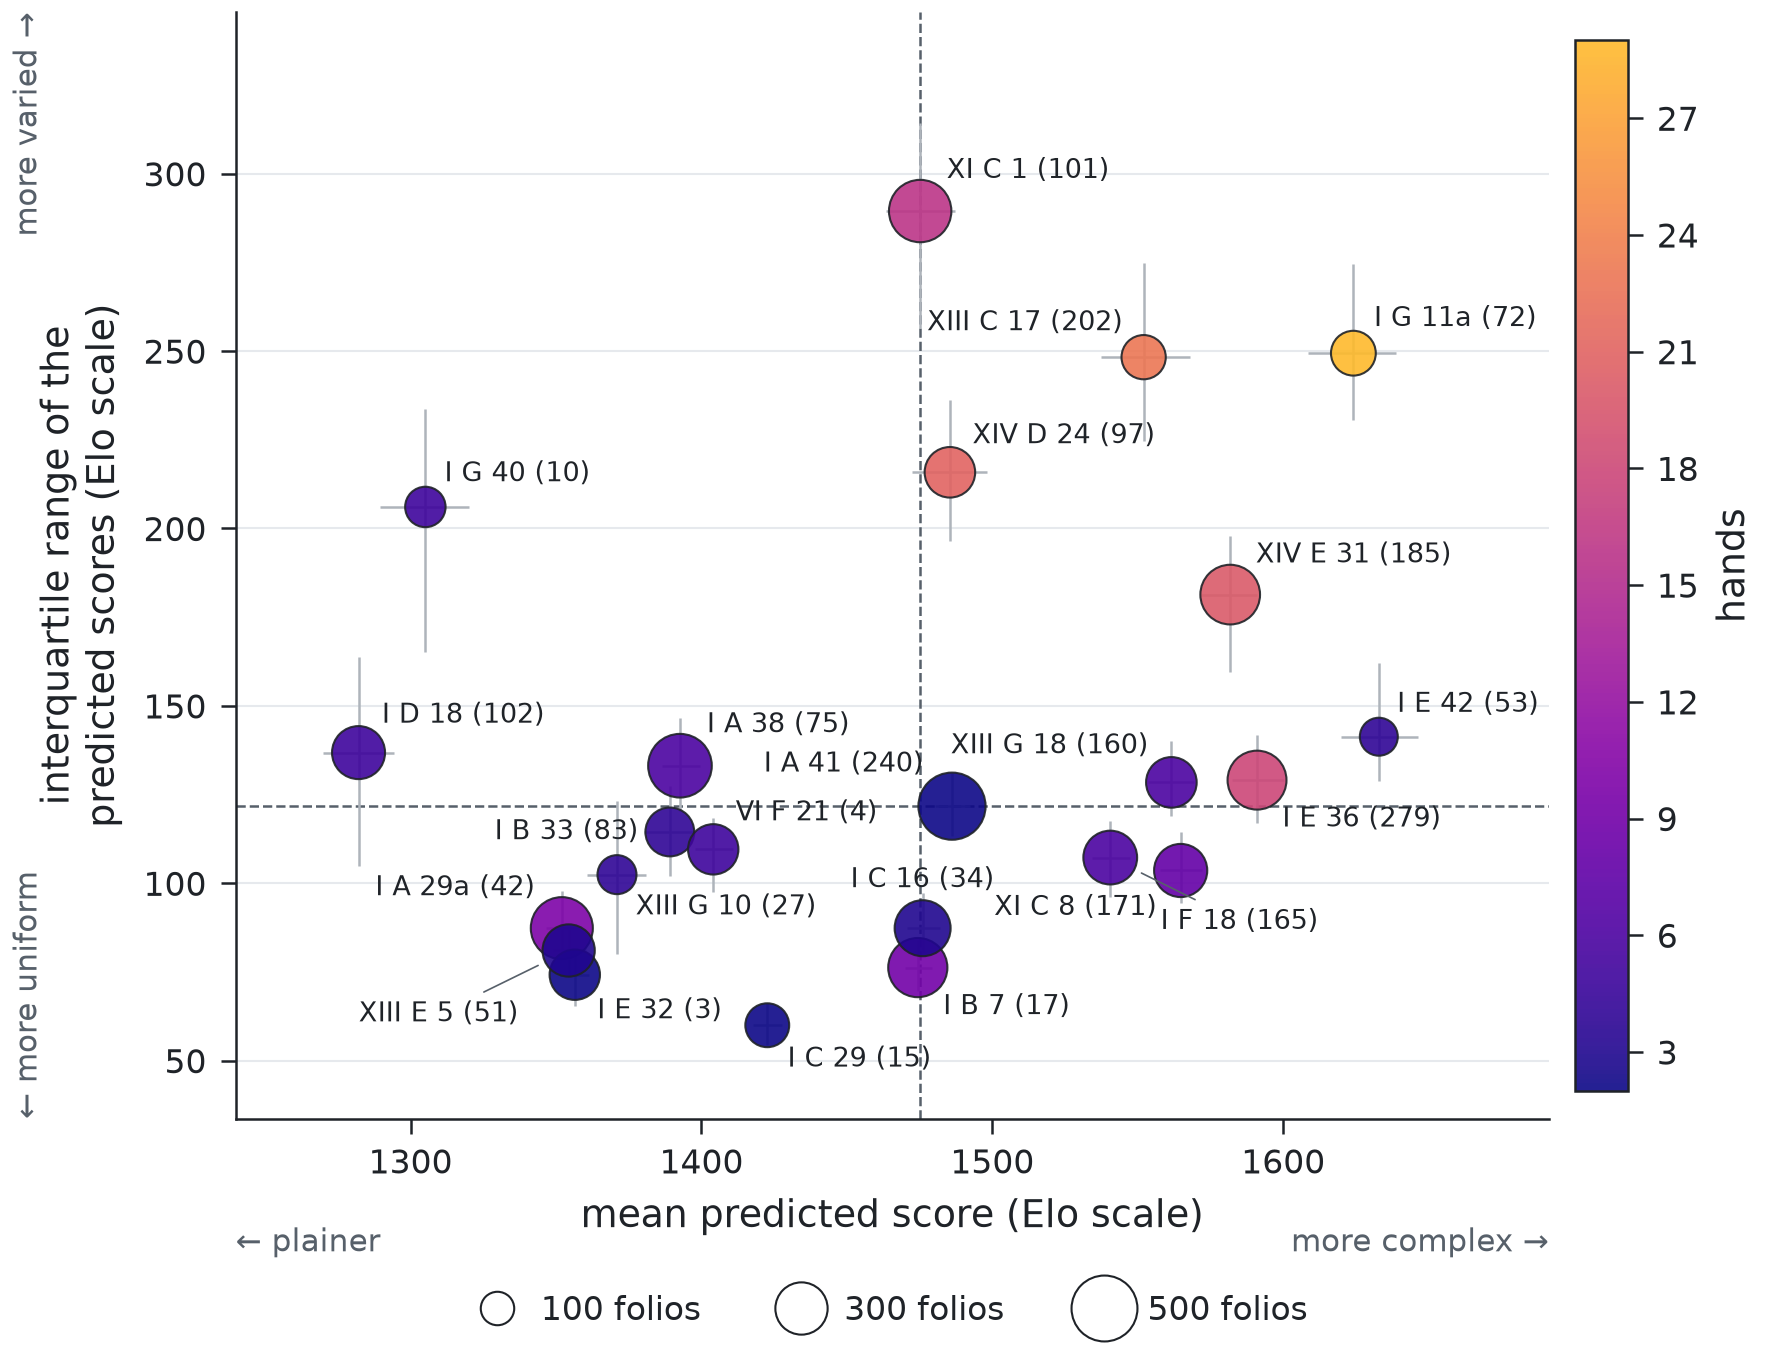
\includegraphics[width=15.00cm]{figures/crux_overview.png}
  \caption{Each manuscript's mean predicted score (horizontal) against the interquartile range of its pages' predicted scores (vertical): how complex its pages are on average, and how much they vary. Points are coloured by the number of hands the catalogue identifies and sized by its number of folios; each is labelled with its shelfmark and, in brackets, the number of texts it holds (counted finely). The dashed lines are the medians of the manuscripts' means and ranges. The whiskers are 95\% intervals from 1,000 resamples of each manuscript's pages. Plain and uniform manuscripts lie towards the lower left, complex and varied ones towards the upper right; plain but varied ones towards the upper left, complex but uniform ones towards the lower right. A page's predicted score is its expected Elo score: the regression of the dataset's Elo scores on the ensemble's out-of-fold scores, 1,500 + 168 $\times$ $z$, $z$ being the page's score under the ensemble of the Layout (geometry) and ViT rankers (equal weights). The rankers were trained without the dataset's pages from XIII G 10, I E 36, I A 29a and I A 38, so every score is out of sample. The 362 leaves on which Kraken finds fewer than 5 text lines (blank or nearly blank) are left out. Catalogue facts from Dragoun, Ebersonová and Doležalová (2021).}
  \label{fig:crux_overview}
\end{figure}
